\chapter{Logical dependencies in key class detection}
\label{cap:key_class_detection}

\section{Introduction and research questions}
\label{sec:key_introduction}
\hspace{4em}Zaidman et al. \cite{ZaidmanJurnal} were the first to introduce the concept of \emph{key classes}, referring to classes found in documents written to provide an architectural overview of the system or an introduction to the system structure.

Key class identification has been previously done using structural dependencies \cite{PagerankENASE}, \cite{enase15}, \cite{PagerankSACI}. In this chapter, key classes are identified using dependencies extracted from the version control system combined with dependencies from the source code. The analysis is performed both separately and together to see how the final results fluctuate depending on the type of dependency used.

The analysis in this chapter is performed on three open-source projects: Ant, Tomcat Catalina, and Hibernate. For this chapter, the following research questions are addressed:

\emph{RQ1: Can combining logical and structural dependencies improve the previous results obtained by using only structural dependencies in key class detection?}  
Since logical dependencies overlap only in a small percentage with structural dependencies, the goal is to combine both dependencies and provide them as input to key class identification tools.

\emph{RQ2: Can logical dependencies alone provide good results in key class detection?}  
This question focuses on using logical dependencies as stand-alone inputs. Although logical dependencies are different than structural dependencies, they may still provide enough system information to be successfully used as input for tools like key classes detection tools.

\emph{RQ3: Does applying the connection strength filter have a positive impact on key class detection?}  
The connection strength filter and the commit size filter will be used to filter co-changes into logical dependencies. The goal is to evaluate whether this new strength filter outperforms the confidence and support filter in key class detection \cite{b4}.






\section{Related work on key class detection} %not refactored
\label{sec:key_related_work}

\hspace{4em}Zaidman et al. \cite{ZaidmanJurnal} were the first to introduce the concept of key classes, referring to classes commonly found in documents that provide an architectural overview of the system or an introduction to its structure. 

Tahvildari and Kontogiannis offered a more detailed definition of key classes: “Usually, the most important concepts of a system are implemented by very few key classes which can be characterized by specific properties. These classes, which we refer to as key classes, manage many other classes or use them in order to implement their functionality. The key classes are tightly coupled with other parts of the system. Additionally, they tend to be rather complex since they implement much of the legacy system’s functionality” \cite{Tahvildari2004ImprovingDQ}.

Other researchers have used similar concepts under different terms, such as important classes \cite{Meyer2014IdentifyingIC} or central software classes \cite{CentralClassesSteidl}. 

Key class identification can be performed using different algorithms and input types. In the research by Osman et al., key class identification is performed using a machine learning algorithm with class diagrams as input \cite{6676885}. Thung et al. build on Osman et al.’s approach by incorporating network metrics and optimistic classification to enhance key class detection \cite{rocclasification}. 

Zaidman et al. \cite{ZaidmanJurnal} apply a web-mining algorithm and dynamic source code analysis to identify key classes. Similarly, Sora et al. use a PageRank-inspired algorithm combined with static source code analysis \cite{PagerankENASE}, \cite{enase15}, \cite{PagerankSACI}. In \cite{Finding-key-classes}, the authors extend this approach by including additional class attributes to improve key class identification. 

The PageRank algorithm, developed initially for ranking web pages \cite{ilprints422}, works based on a recommendation system. If one node is connected to another, it recommends the second node. In previous studies, connections were based on structural dependencies extracted from static code analysis. If class A has a structural dependency with class B, both A and B recommend each other.

Based on their importance, the ranking algorithm assigns a score to all classes from the analyzed system's source code. To distinguish important classes from the rest, a threshold for the TOP-ranked classes is set. The TOP threshold value can range from 1 to the total number of classes in the system. 

Some researchers \cite{ZaidmanJurnal}, \cite{Ding2016AnIA}, \cite{PAN2018188} suggest that 15\% of the total number of classes in the system is a suitable value for the TOP threshold. Others \cite{Finding-key-classes} argue that 15\% is too high and propose a range of 20 to 30 classes as a more appropriate threshold \cite{b4}.

\section{Methodology and implementation}
\label{sec:key_methodology_implementation}

This section presents the methodology and implementation used for key class detection. Section \ref{subsec:key_evalmetrics} describes the evaluation metrics used to assess the results of detected key classes. Section \ref{subsec:key_previous_measurements} describes the baseline approach by Şora et al. \cite{Finding-key-classes}. Section \ref{subsec:key_current_approach} describes the current approach, which extends the baseline by incorporating logical dependencies from the version control system. Section \ref{subsec:key_tool} describes the tool setup and workflow used for extracting, filtering, and processing logical dependencies and using them for key class detection.


\subsection{Metrics for results evaluation} %not refactored
\label{subsec:key_evalmetrics}

\hspace{4em}To evaluate the quality of the key classes ranking algorithm and solution produced, the key classes found are compared with a reference solution.

The reference solution is extracted from the developer documentation. Classes mentioned in the documentation are considered key classes and form the reference solution (ground truth) used for validation \cite{7551990}. A classification model is then used to compare the two solutions. The quality of the solution produced is evaluated by using metrics that evaluate the performance of the classification model, such as Precision-Recall and Receiver Operating Characteristic Area Under Curve (ROC-AUC). 

A classification model (or "classifier") is a mapping between expected results and predicted results \cite{ROCIntro}, \cite{ROCBRADLEY19971145}. Both results can be labeled as positive or negative, which leads us to the confusion matrix from figure \ref{fig:confusion} \cite{b4}. 
\begin{figure}[h]
\centering
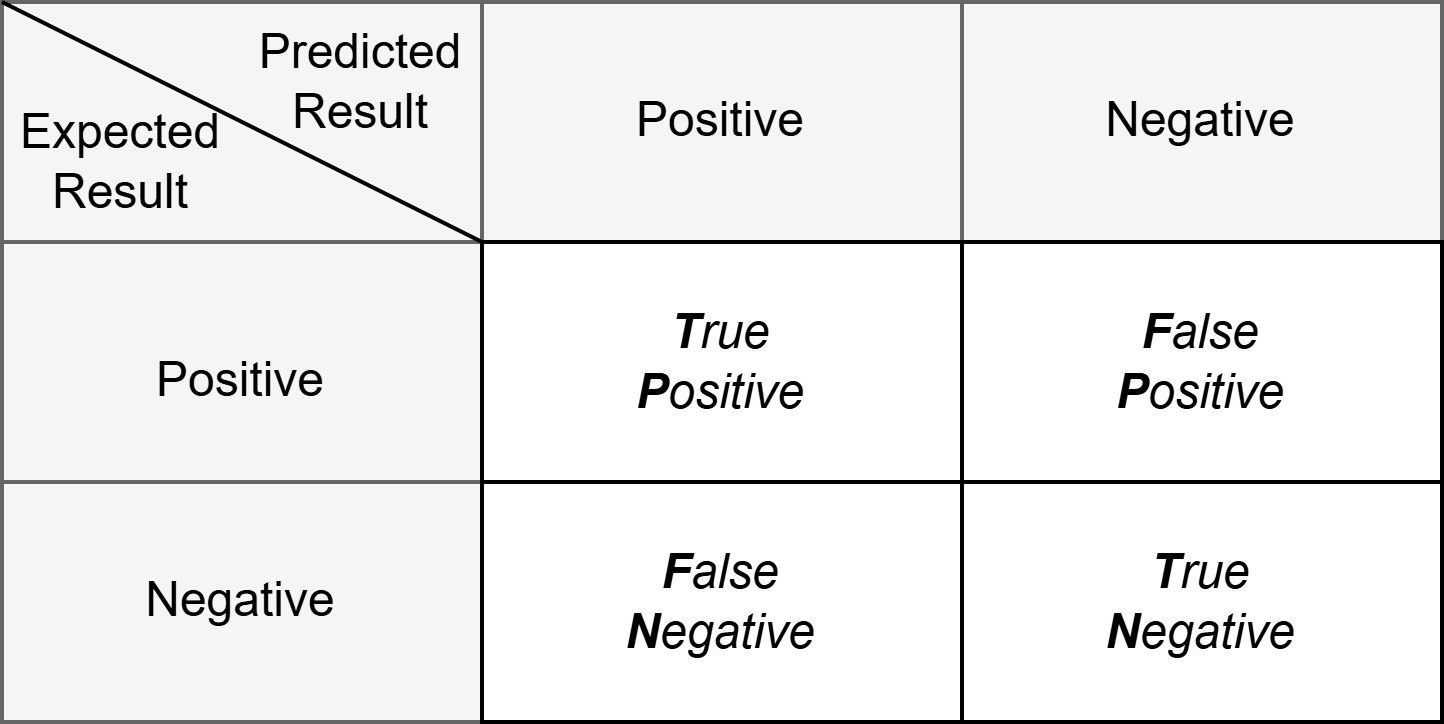
\includegraphics[scale=0.9]{confusion.png}
\caption{Confusion matrix}
\label{fig:confusion}
\centering
\end{figure}
The confusion matrix has the following outcomes:\\
- \textit{true positive}, if the expected result is positive and the predicted result is also positive.\\
- \textit{false positive}, if the expected result is positive but the predicted result is negative.\\
- \textit{false negative}, if the expected result is negative but the predicted result is positive.\\
- \textit{true negative}, if the expected result is negative and the predicted result is also negative.



\underline{\textit{Precision-recall}}


\hspace{-4em}Precision is the ratio of True Positives to all the positives of the result set.

\begin{equation}
 precision = \frac{TP}{TP+FN}
\end{equation}
The recall is the ratio of True Positives to all the positives of the reference set.

\begin{equation}
 recall = \frac{TP}{TP+FP}
\end{equation}

To distinguish the key classes from the rest of the classes a TOP threshold is used. Some researchers consider that 15\% of the total classes is the best value for the TOP threshold and others consider that the value should be in the range of 20-30. 

The precision-recall metric is suited if the threshold value is fixed. If the threshold value is variable, then metrics that capture the behavior over all possible values must be used. Such metric is the Receiver Operating Characteristic metric.

\underline{\textit{Receiver Operating Characteristic Area Under Curve}}


The ROC graph is a two-dimensional graph that has on the X-axis plotted the false positive rate and on the Y-axis the true positive rate. By plotting the true positive rate and the false positive rate at thresholds that vary between a minimum and a maximum possible value we obtain the ROC curve. The area under the ROC curve is called Area Under the Curve (AUC).

The true positive rate (TPR) of a classifier is calculated as the division between the number of true positive results identified and all the positive results identified:

\begin{equation}
TPR = \frac{TP}{TP+FN}
\end{equation}
The false positive rate (FPR) of a classifier is calculated as the division between the number of false positive results identified and all the negative results identified:

\begin{equation}
FPR = \frac{FP}{FP+TN}
\end{equation}


The True Positives (TP) are the classes found in the reference solution and in the top TOP ranked classes. False Positives (FP) are the classes not found in the reference solution but in the TOP ranked classes.
True Negatives (TN) are classes found neither in the reference solution nor in the TOP ranked classes. False Negatives (FN) are classes found in the reference solution but not in the TOP ranked classes.

In related research, the ROC-AUC metric has been used to evaluate the results for finding key classes of software systems. For a classifier to be considered good, its ROC-AUC metric value should be as close to 1 as possible.
When the value is 1, then the classifier is considered to be perfect. A metric value between 0.8 and 0.9 means that the classifier is excellent. Between 0.8 and 0.7 means acceptable results, and between 0.7 and 0.5 means poor results \cite{ROC_METRIC_VALS, b4}. 



\subsection{Baseline approach}
\label{subsec:key_previous_measurements}

\hspace{4em}We use the research of I. Şora et al. \cite{Finding-key-classes} as a baseline for our research involving the usage of logical dependencies to find key classes. The entire workflow of the baseline approach is also presented in figure \ref{fig:baseline_approach}.

\begin{figure}[H]
\centering
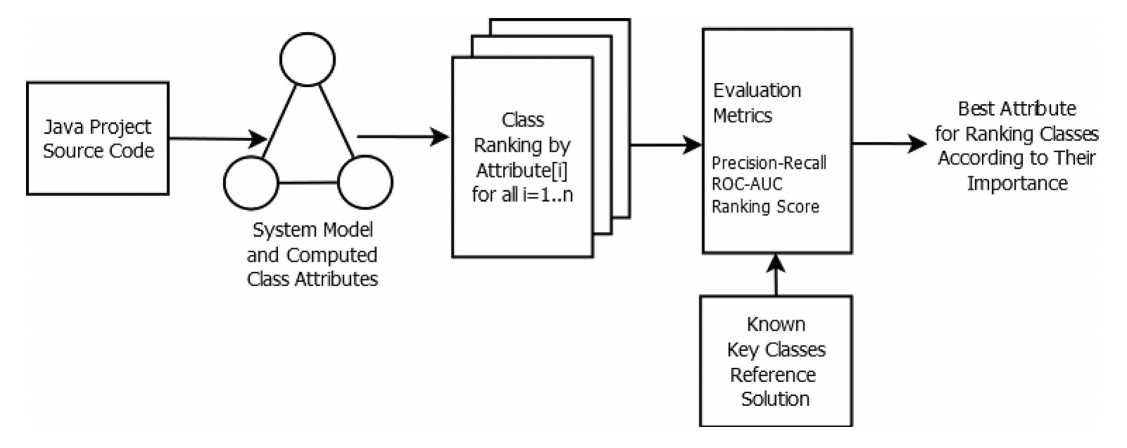
\includegraphics[width=\textwidth]{baseline_approach.PNG}
\caption{Overview of the baseline approach. Reprinted from “Finding key classes in object-oriented
software systems by techniques based on static analysis.” by Ioana Sora and Ciprian-Bogdan Chirila, 2019, Information and Software Technology, 116:106176. Reprinted with permission. }
\label{fig:baseline_approach}
\centering
\end{figure}


Şora et al. used static source code analysis, a page ranking algorithm, and additional class attributes to identify key classes \cite{PagerankENASE, enase15, PagerankSACI, Finding-key-classes}. The page ranking algorithm is a customized version of PageRank, originally developed for ranking web pages \cite{ilprints422}. It operates based on a recommendation system: if one node is connected to another, it recommends the second node. In this context, connections are established through structural dependencies. For example, if class A has a structural dependency with class B, both A and B recommend each other.

The ranking algorithm evaluates all classes from the system’s source code based on their importance. To identify the key classes from the rest, a threshold is set for the highest-ranked classes. This threshold, referred to as the TOP threshold, can range from 1 to the total number of classes in the system \cite{b4}. In the baseline approach, the TOP threshold is typically set between 20 and 30 classes.


The baseline approach involves a tool that processes the system’s source code to identify key classes and compares the results with a reference solution extracted from the developer documentation using a classification model. To rank classes by importance, various class metrics are considered \cite{Ding2016AnIA, ZaidmanJurnal, PAN2018188}. Below are some key class metrics used in the baseline approach for ranking.

\textbf{Class attributes that characterize key classes}


The metrics used in the baseline research can be grouped into the following categories: 

\begin{itemize}
	\item class size metrics: number of fields (NoF),  number of methods (NoM), global size (Size = NoF+NoM).
	\item class connection metrics, any structural dependency between two classes:
		\begin{itemize}
			\item CONN-IN, the number of distinct classes that use a class;
			\item CONN-OUT, the total number of distinct classes that are used by a class;
			\item CONN-TOTAL, the total number of distinct classes that a class uses or are used by a class (CONN-IN + CONN-OUT).
			\item CONN-IN-W, the total weight of distinct classes that use a class. 
			\item CONN-OUT-W, the total weight of distinct classes that are used by a class. 
			\item CONN-TOTAL-W, the total weight of all connections of the class (CONN-IN-W + CONN-OUT-W) \cite{Finding-key-classes}.
		\end{itemize}
	\item class pagerank values, previous research use pagerank values computed on both directed and undirected, weighted and unweighted graphs:
		\begin{itemize}
			\item PR - value computed on the directed and unweighted graph;
			\item PR-W - value computed on the directed and weighted graph;
			\item PR-U - value computed on the undirected and unweighted graph;
			\item PR-U-W - value computed on the undirected and weighted graph;
			\item PR-U2-W - value computed on the weighted graph with back-recommendations \cite{PagerankENASE}, \cite{enase15}, \cite{Finding-key-classes}, \cite{PagerankSACI}.
		\end{itemize}
\end{itemize}


Due to the fact that the TOP threshold is varied, the Receiver Operating Characteristic Area Under Curve metric is used for the evaluation of the results.



\subsection{Current approach}
\label{subsec:key_current_approach}

\hspace{4em}The baseline approach uses a tool that takes as an input the source code of the system and applies ranking strategies to rank the classes according to their importance. We modified the tool used by the baseline approach to take also the logical dependencies as input; the rest of the workflow is the same as in the baseline approach (figure \ref{fig:baseline_approach}).
\begin{figure}[H]
\centering
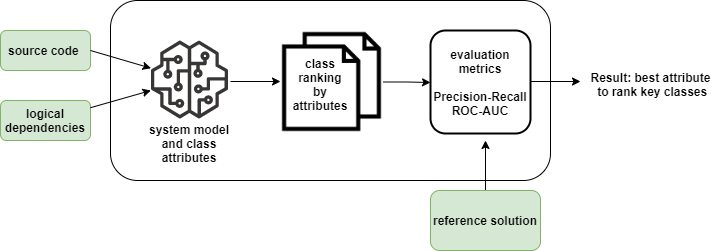
\includegraphics[scale=0.43]{current_approach.PNG}
\caption{Overview of the current approach.}
\label{fig:baseline_approach}
\end{figure}

Below are some of the class metrics used in the baseline approach and in our current research to rank the classes according to their importance. The class metrics used can be separated into two categories: class connection metrics and class PageRank values. The class connection metrics are CONN-TOTAL-W, which is the total weight of all connections of the class, and CONN-TOTAL, the total number of distinct classes that a class uses or is using the class \cite{Finding-key-classes}.

Previous research used PageRank values computed on both directed and undirected, weighted and unweighted graphs. In the current research, we use the PR, which is the PageRank value computed on the directed and unweighted graph, the PR-U, which is the value computed on the undirected and unweighted graph, and the PR-U2-W, the value computed on the weighted graph with back-recommendations \cite{PagerankENASE}, \cite{enase15}, \cite{Finding-key-classes}, \cite{PagerankSACI}.

The comparison between the current proposed approach and the baseline method is illustrated in Figure \ref{fig:baseline_comparison}. 
\begin{figure}[H]
\centering
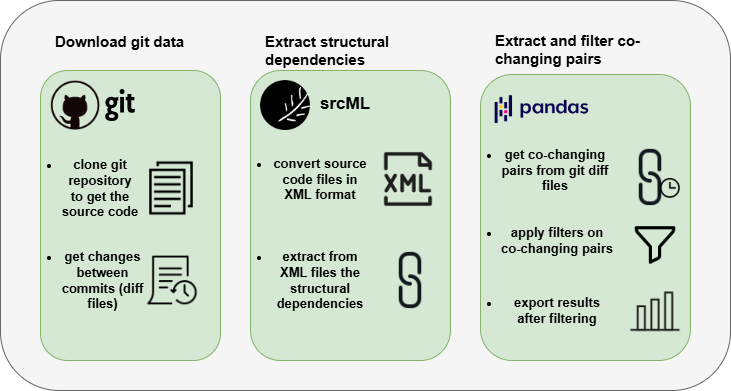
\includegraphics[width=\textwidth]{baseline_comparison.png}
\caption{ Comparison between the new approach and the baseline }
\label{fig:baseline_comparison}
\centering
\end{figure}


\subsection{Tool setup and current workflow used}
\label{subsec:key_tool}

\hspace{4em}The entire process of extracting co-changing pairs from the versioning system, filtering them, and exporting the remaining pairs is performed using the same Python tool described and used in Chapters \ref{extraction} and \ref{chap:combining_dependencies}. The entire tool workflow is presented in Figure \ref{fig:workflow_key}.

\begin{figure}[H]
\centering
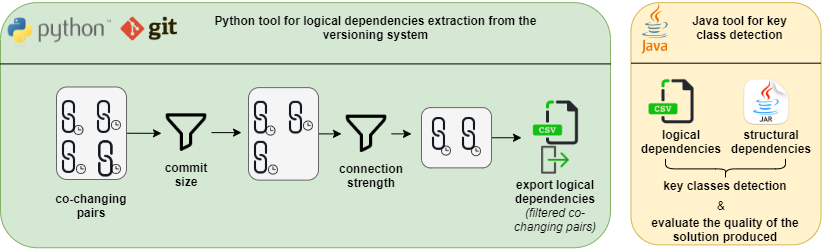
\includegraphics[width=\textwidth]{key_class_workflow.png}
\caption{Workflow for key classes detection}
\label{fig:workflow_key}
\centering
\end{figure}`


The filtering process involves applying two filters: the commit size filter and the connection strength filter. The commit size filter excludes all commits with more than 10 files \(cs \leq 10\). The connection strength filter ranges from \( \geq 10\% \) to \( \geq 100\% \), with a step of 10, resulting in 10 different sets of logical dependencies, each corresponding to a specific strength threshold. A fixed threshold is not used because the goal is to assess how strength thresholds impact key class detection results. After filtering, the remaining co-changing pairs are exported to CSV files.

The next step is to use the exported logical dependencies for key class detection. The same key class detection tool described in Section \ref{subsec:key_previous_measurements} is used, with adaptations to support logical dependencies. Previously, the tool processed only structural dependencies extracted from the system's source code. The tool ranks the top key classes and evaluates the results using the ROC-AUC metric.





\section{Data set used in experimental analysis}
\label{sec:key_dataset}


The research of I. Sora et al \cite{Finding-key-classes} takes into consideration structural public dependencies that are extracted using static analysis techniques and was performed on the object-oriented systems presented in table \ref{tab:keyclass:overview}.

The requirements for a system to qualify as suited for investigations using logical dependencies are: has to be on GitHub, has to have release tags to identify the version, and also has to have an increased number of commits. 
From the total of 14 object-oriented systems listed in the paper \cite{Finding-key-classes}, 13 of them have repositories in Github \ref{tab:gitfoundsystems}. And from the found repositories we identified only 6 repositories that have the same release tag as the specified version from table \ref{tab:keyclass:overview}. It is important to identify the correct release tag for each repository to limit the commits further analyzed by date. Only commits that were made until the specified release are considered and analyzed.
The commits number found on the remaining 6 repositories varies from 19108 commits for Tomcat Catalina to 149 commits for JHotDraw. In order to have more accurate results, we need a significant number of commits, so we reached the conclusion that only 3 systems can be used for key classes detection using logical dependencies: Apache Ant, Hibernate, and Tomcat Catalina.  From all the systems mentioned in table \ref{tab:keyclass:overview} Apache Ant is the most used and analyzed in other  works \cite{enase19}, \cite{7332515}, \cite{1402122}, \cite{Kamran2016IdentificationOC}.

\begin{table}[H]
\renewcommand{\arraystretch}{1}
\caption{Analyzed software systems in previous research paper.}
\label{tab:keyclass:overview}
\centering
\resizebox{\textwidth}{!}{
\begin{tabular}{|c|c|p{7cm}|c|}
\hline
ID	&	System	&	Description	&	Version	\\
\hline
Sl	&	Apache Ant	&	Java library and command line tool that drive the build processes as targets and extension points depending upon each other	&	1.6.1	\\ \hline
S2	&	Argo UML	&	UML modelling tool with support for all UML diagrams.	&	0.9.5	\\ \hline
S3	&	GWT Portlets	&	Open source web framework for building GWT (Google Web Toolkit) Applications.	&	0.9.5 beta	\\ \hline
S4	&	Hibernate 	&	Persistence framework for Java.	&	5.2.12	\\ \hline
S5	&	javaclient	&	Java distributed application for playing with robots	&	2.0.0	\\ \hline
S6	&	jEdit	&	Java mature text editor for programmers.	&	5.1.0	\\ \hline
S7	&	JGAP	&	Genetic Algorithms and Genetic Programming Java library.	&	3.6.3	\\ \hline
S8	&	JHotDraw	&	JHotDraw is a two-dimensional graphics framework for structured drawing editors that is written in Java.	&	6.0b.1	\\ \hline
S9	&	JMeter	&	JMeter is a Java application designed to load test functional behavior and measure performance	&	2.0.1	\\ \hline
S10	&	Log4j	&	Logging Service	&	2.10.0	\\ \hline
S11	&	Mars	&	The Mars Simulation Project is a Java project that models and simulates human settlements on Mars planet	&	3.06.0	\\ \hline
S12	&	Maze	&	The Maze-solver project simulates an artificial intelligence algorithm on a maze	&	1.0.0	\\ \hline
S13	&	Neuroph	&	Neuroph is a Java neural network framework.	&	2.2.0	\\ \hline
S14	&	Tomcat Catalina	&	The Apache Tomcat project is an open-source implementation of JavaServlet and JavaServerPages technologies	&	9.0.4	\\ \hline
S15	&	Wro4J	&	The Wro4J is a web resource (JS and CSS) optimizer for Java.	&	1.6.3	\\ 
\hline
\end{tabular}
}
\end{table}



\begin{table}[H]
\renewcommand{\arraystretch}{1}
\caption{Found systems and versions of the systems in GitHub. }
\label{tab:gitfoundsystems}
\centering
\scalebox{0.8}{
\begin{tabular}{|c|c|c|c|c|}
\hline
ID	&	System	&	Version	&	Release Tag name	&	Commits number	\\
\hline
\rowcolor{lightgreen}
Sl	&	Apache Ant	&	1.6.1	&	rel/1.6.1	&	6713	\\
S2	&	Argo UML	&	0.9.5	&	not found	&	0	\\
S3	&	GWT Portlets	&	0.9.5 beta	&	not found	&	0	\\
\rowcolor{lightgreen}
S4	&	Hibernate 	&	5.2.12	&	5.2.12	&	6733	\\
S5	&	javaclient	&	2.0.0	&	not found	&	0	\\
S6	&	jEdit	&	5.1.0	&	not found	&	0	\\
S7	&	JGAP	&	3.6.3	&	not found	&	0	\\
S8	&	JHotDraw	&	6.0b.1	&	not found	&	149	\\
S9	&	JMeter	&	2.0.1	&	v2\_1\_1	&	2506	\\
S10	&	Log4j	&	2.10.0	&	v1\_2\_10-recalled	&	634	\\
S11	&	Mars	&	3.06.0	&	not found	&	0	\\
S12	&	Maze	&	1.0.0	&	not found	&	0	\\
S13	&	Neuroph	&	2.2.0	&	not found	&	0	\\
\rowcolor{lightgreen}
S14	&	Tomcat Catalina	&	9.0.4	&	9.0.4	&	19108	\\
S15	&	Wro4J	&	1.6.3	&	v1.6.3	&	2871	\\
\hline
\end{tabular}
}
\end{table}


Figures \ref{fig:strength_overview_ant}, \ref{fig:strength_overview_hibernate} and \ref{fig:strength_overview_catalina} intend to offer a big picture of systems. The dots represent the maximum number of updates of one entity with another, and the black line represents the average occurrence value of the system.
It can be observed that all systems have multiple entities that update only once, meaning that we might have many confidence values of 1 (the highest value possible) for entities that update only once together. 
We plotted only the maximum occurrences between entities to not overcrowd the plot. Even with only the maximum occurrences plotted, it can be observed that most of the points are at the bottom of the graphic. So, plotting all the points wouldn't change the overall picture of the system. The excluded points will only create a line of points even lower at the bottom of the graphic.

\begin{figure}
\centering
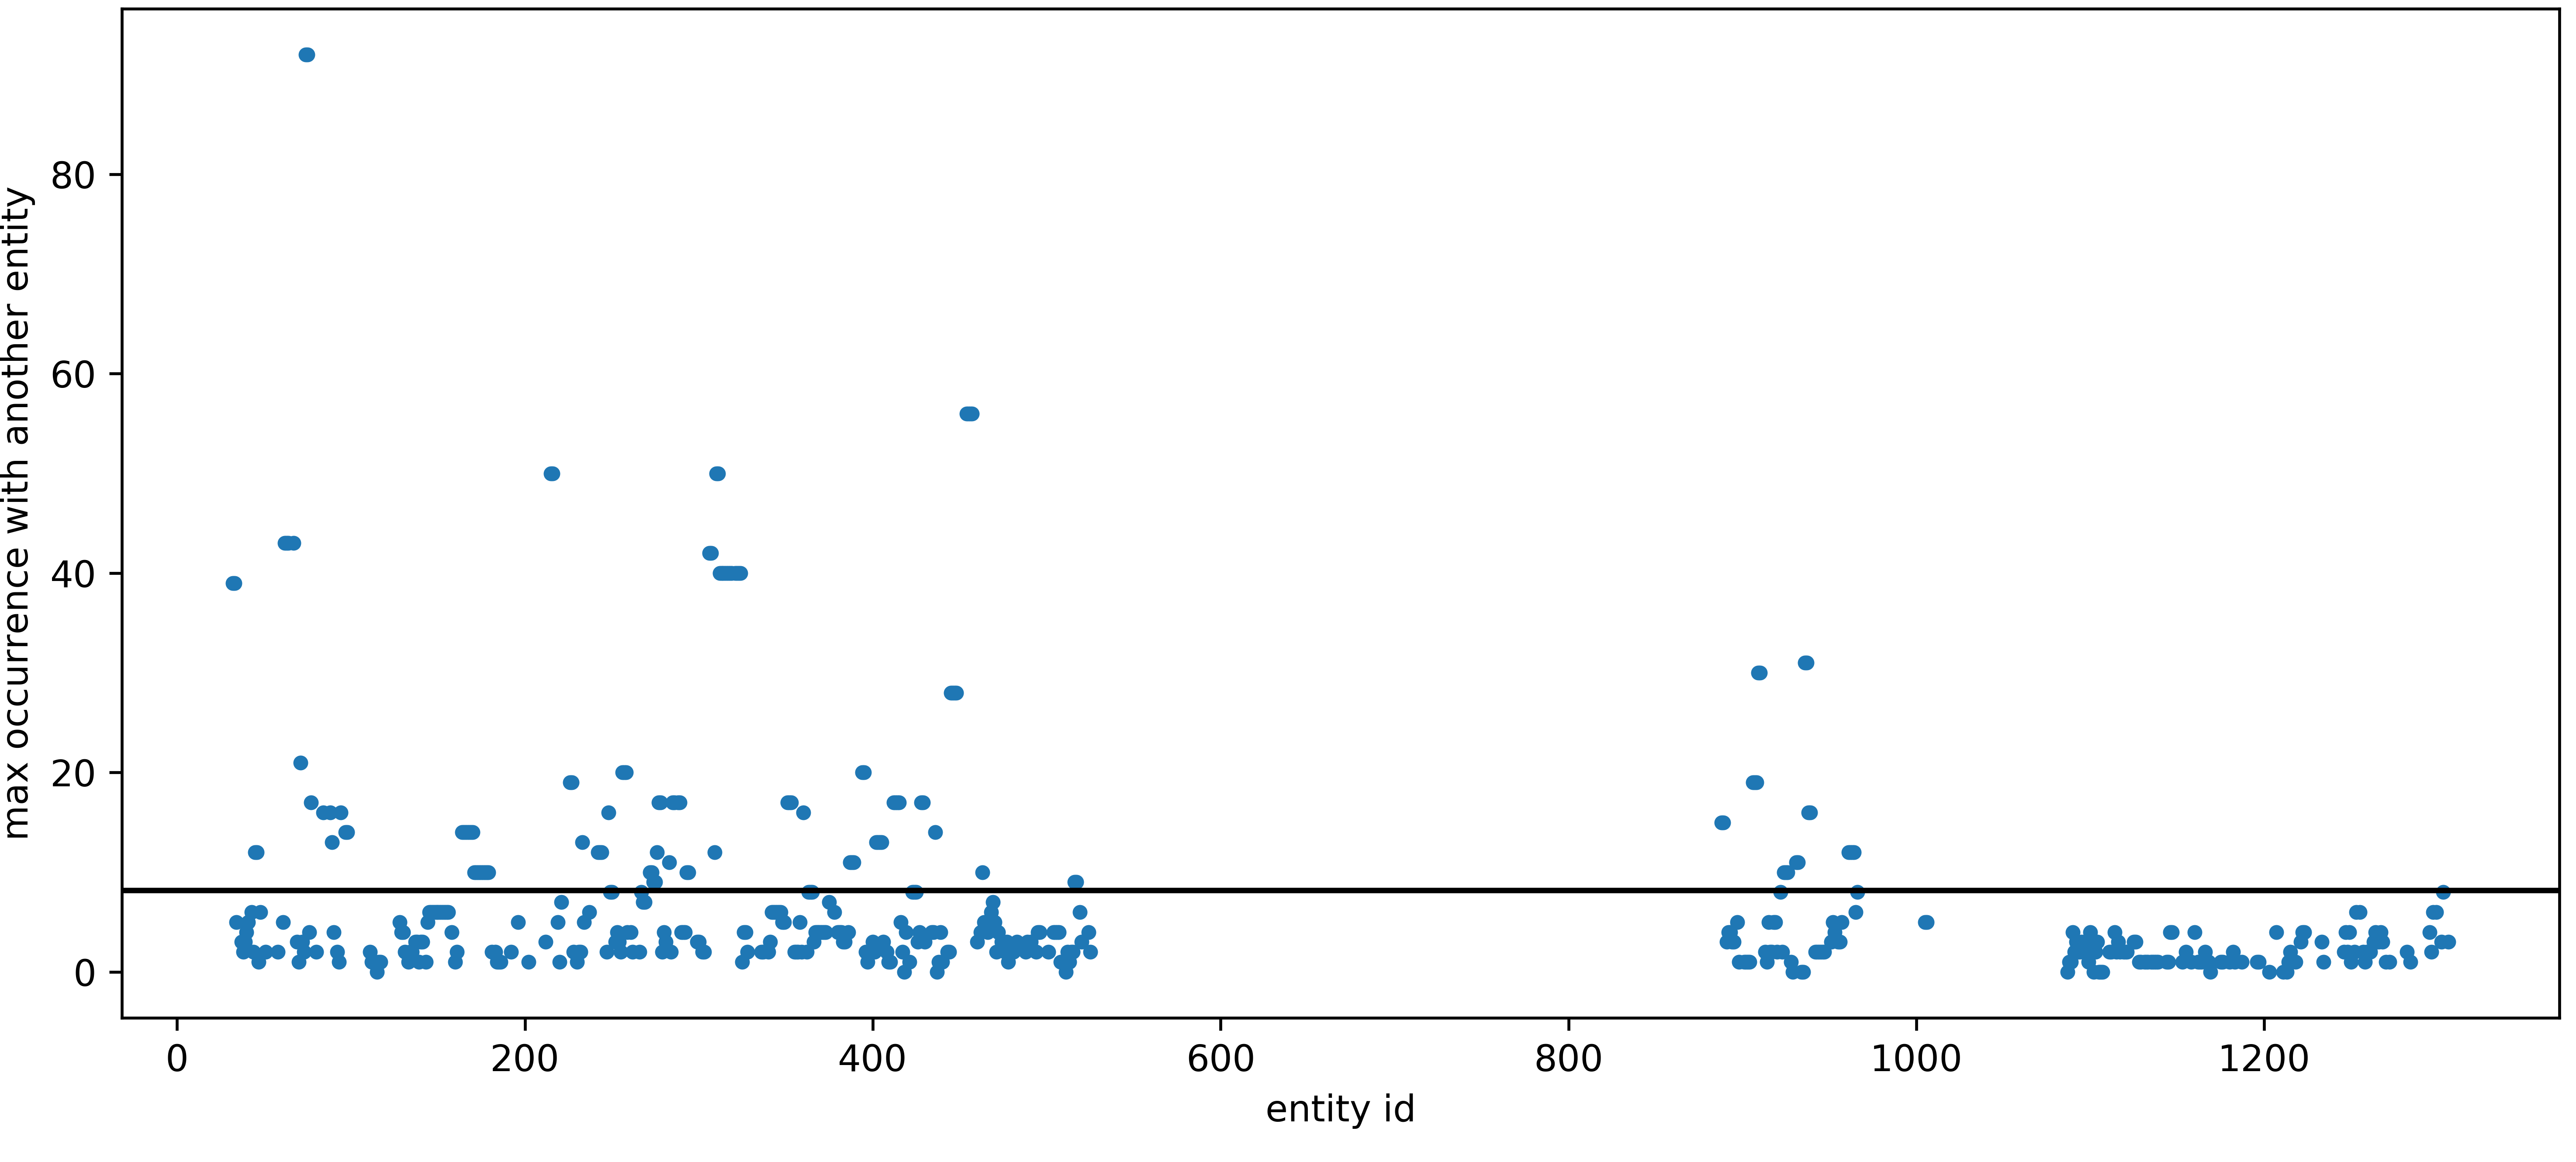
\includegraphics[width=\textwidth]{fig_ant_maxOcc.png}
\caption{Overview of the number of occurrences in Ant. }
\label{fig:strength_overview_ant}
\centering
\end{figure}

\begin{figure}
\centering
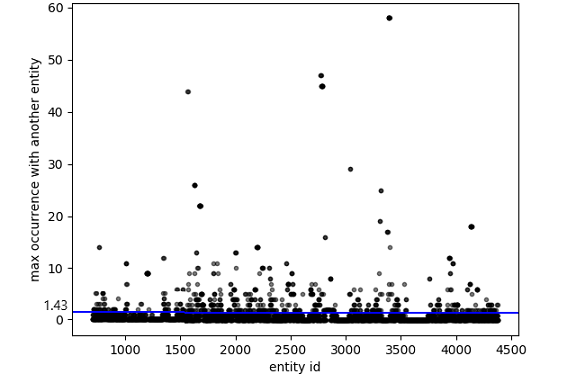
\includegraphics[width=\textwidth]{fig_hibernate_maxOcc.png}
\caption{Overview of the number of occurrences in Hibernate. }
\label{fig:strength_overview_hibernate}
\centering
\end{figure}

In figure \ref{fig:strength_overview} we plotted for two systems (one small-sized and one medium-sized) the number of structural dependencies, co-changing pairs before filtering, and co-changing pairs after filtering. With the connection strength filter, the small-sized system didn't lose all the co-changing pairs once with the filtering.
We compare the number of remaining co-changing pairs with the number of structural dependencies because, according to surveys \cite{Shtern:2012:CMS:2332427.2332428}, \cite{sar}, the main reason why logical dependencies (filtered co-changes) are not used together with structural dependencies is their size. So, it is essential to get an overview of the comparison between the number of co-changing pairs and the number of structural dependencies at each filtering step.

We call the co-changing pairs that remain after filtering, logical dependencies. 
After this step, we will use the logical dependencies obtained with different threshold values and see which threshold value performs the best. Up until now, we only looked at the size of the resulting logical dependencies and decided if a filter and its threshold are good or not. Now, we can also look at the results obtained by using the logical dependencies and decide.

\begin{figure}
\centering
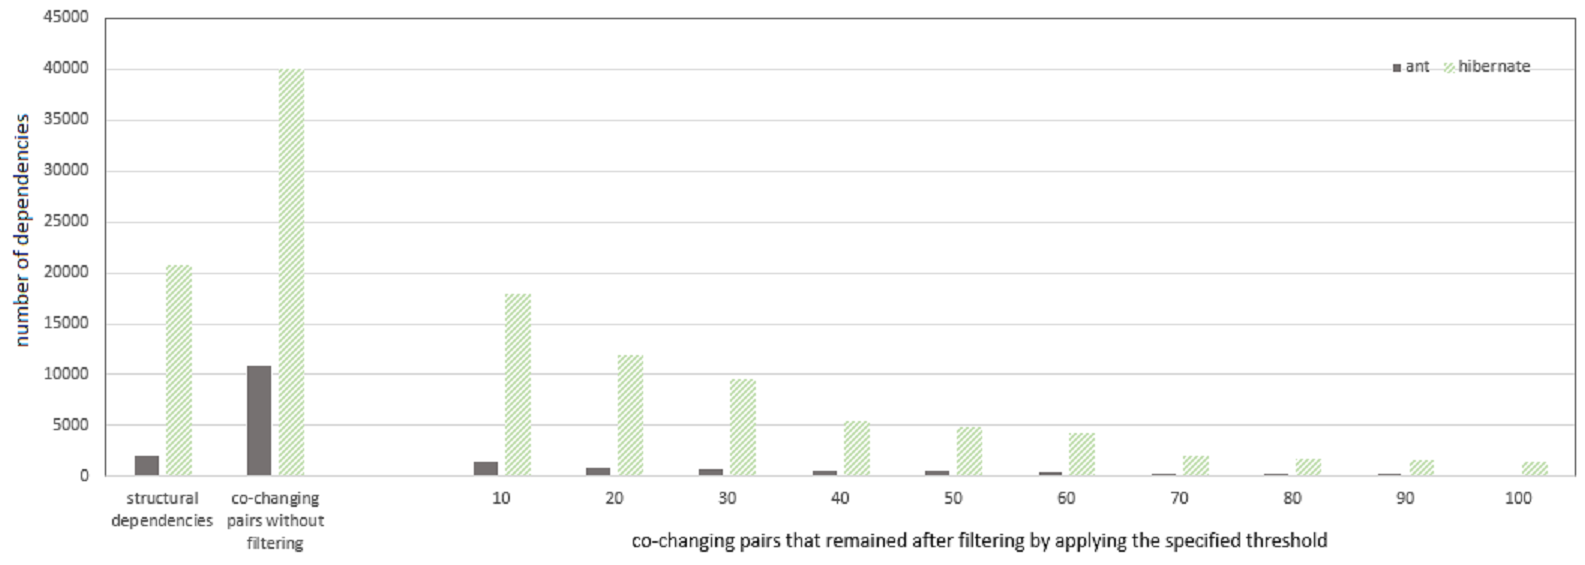
\includegraphics[width=\textwidth]{strength_overview.PNG}
\caption{Overview of the impact of connection strength filtering on the number of co-changing pairs. }
\label{fig:strength_overview}
\centering
\end{figure}

\section{Experimental plan and results}
\label{sec:key_plan_and_results}

As presented in section \ref{sec:baseline_approach}, the key class detection was previously done only by using the structural dependencies of the system. 
In this section, we use the same tool used in the baseline approach presented in section \ref{sec:baseline_approach}, and we add a new input to it, the logical dependencies. 

In subsection \ref{sec:dataset}, we present the data set used to generate new results and, in subsection \ref{sec:measure_baseline}, we present the previously obtained results. Subsection \ref{sec:measure_ld_sd} presents the conclusions and results obtained by using logical and structural dependencies together, and subsection \ref{sec:measure_ld} presents the conclusions and results obtained by using only logical dependencies. Subsection \ref{sec:measure_metrics} presents a comparison between results obtained with the confidence metric versus results obtained with the strength metric. And finally, subsection \ref{sec:compare_others} presents a comparison between the results obtained in the current paper and the results of other researchers.


\subsection{Experimental plan}
\label{subsec:key_plan}

Our study aims to check whether logical dependencies can be usable. Previous research focused on filtering the co-changes extracted from the versioning system and studying how filtering affects their size or how they overlap with structural dependencies. We intend to use the resulting information after co-changes filtering (the logical dependencies) in a tool that usually receives structural dependencies as input.

Our research questions are the following: \textbf{RQ1:} \textit{Can logical dependencies combined with structural dependencies enhance the results obtained by using only structural dependencies in key class detection?} \textbf{RQ2:} \textit{Can logical dependencies provide good results if they are used instead of structural dependencies in key class detection?} \textbf{RQ3:} \textit{ Does the connection strength filter has a favorable impact on the detection of key classes?}

To answer the research questions, we defined the following experimental plan: 
We will use the tool mentioned in the above section. Previously the tool had as input the structural dependencies of the system and the reference solution, and the output was the ROC-AUC score. The closer the ROC-AUC score is to 1, the better the results.  
With the slightly modified version of the tool, we are able to receive as input also logical dependencies.


For \textbf {RQ1}, we will give as input to the tool the structural and the logical dependencies, and we will compare the ROC-AUC scores obtained with the results obtained by using only structural dependencies.


\noindent\fbox{%
    \parbox{\textwidth}{%
      \textit{Hypothesis:} Key classes detection is better when we provide both types of dependencies as input to the tool. The output has a higher ROC-AUC score than the base approach.
    }%
}
\medskip

Our findings for this research question can be found in section \ref{sec:measure_ld_sd}.


For \textbf {RQ2}, we will give as input to the tool only logical dependencies, and we will compare the ROC-AUC scores obtained with the results obtained by using only structural dependencies, and by using structural and logical dependencies combined.
We do not expect that the results will be better compared to the results previously obtained, but we expect results that have a ROC-AUC score close to those values. That would mean that logical dependencies can provide enough information to detect most of the key classes of the system.

\medskip

\noindent\fbox{%
    \parbox{\textwidth}{%
      \textit{Hypothesis:} The output has a ROC-AUC score between 0.7 and 1. 
    }%
}

\medskip

Our findings for this research question can be found in section \ref{sec:measure_ld}.

For \textbf {RQ3}, we will generate two sets of logical dependencies. One set will be generated with the connection strength filter and one with the confidence filter. We will then use each set in two different scenarios: one when we only use logical dependencies to detect key classes and one when we use logical and structural dependencies for detection. Finally, we will compare the results obtained. We expect that the connection strength filter will generate better results. 

\medskip

\noindent\fbox{%
    \parbox{\textwidth}{%
      \textit{Hypothesis:} The results obtained by using the connection strength filter are better than the ones obtained with the confidence filter. 
    }%
}

\medskip
Our findings for this research question can be found in section \ref{sec:measure_metrics}.


\subsection{Results using only the baseline approach}
\label{subsec:key_results_baseline}

In table \ref{tab:previousresults} are presented the ROC-AUC values for different attributes computed for the systems Ant, Tomcat Catalina, and Hibernate by using the baseline approach. We compare these values with the new values obtained by using also logical dependencies in key class detection.

\begin{table}
\renewcommand{\arraystretch}{1}
\caption{ROC-AUC metric values extracted. }
\label{tab:previousresults}
\centering
\scalebox{0.9}{
\begin{tabular}{|c|ccc|}
\hline
Metrics &	Ant	&	Tomcat Catalina	&	Hibernate	\\
\hline

PR\_U2\_W	&	0.95823	&	0.92341	&	0.95823	\\
PR	&	0.94944	&	0.92670	&	0.94944	\\
PR\_U	&	0.95060	&	0.93220	&	0.95060	\\
CONN\_TOTAL\_W	&	0.94437	&	0.92595	&	0.94437	\\
CONN\_TOTAL	&	0.94630	&	0.93903	&	0.94630	\\
\hline
\end{tabular}
}
\end{table}

\subsection{Results using combined structural and logical dependencies}
\label{subsec:key_results_combined}

The tool used in the baseline approach runs a graph-ranking algorithm on a graph that contains all the structural dependencies extracted from static source code analysis.
Each edge in the graph represents a dependency. The entities that form a structural dependency are represented as vertices in the graph. 
As mentioned in section \ref{sec:baseline_approach}, we modified the tool to take structural and logical dependencies as input.
For this subsection's measurements, we add the logical dependencies in the graph that contains all structural dependencies. Since it is a weighted graph, if a structural dependency is also a logical dependency, then the final weight of the connection is the sum of the weight computed for the structural dependency and the connection strength metric associated with the logical dependency.

In tables \ref{tab:measurementscombined:ant}, \ref{tab:measurementscombined:tomcat}, and \ref{tab:measurementscombined:hibernate}, on each line, we have the computed the key class metric generated with logical dependencies extracted with the connection strength threshold that is specified in the colums header.

We started with logical dependencies that have a connection strength metric greater than 10, then we repeatedly increased the value by 10 until we reached 100. The last column of the table contains the results previously obtained by the tool by only using structural dependencies (the results presented in section \ref{sec:measure_baseline}). So, to answer \textit{RQ1: Can logical dependencies combined with structural dependencies enhance the results obtained by using only structural dependencies in key class detection?}: The results obtained by combining structural and logical dependencies are close to the previously registered values but, in most cases, do not surpass them. Underlined are the values that are better than the previously registered values. We can observe that for all 3 systems, the best values obtained are for connection strength between 40-70.

\begin{table}[!h]
\setlength\tabcolsep{3.5pt}
\caption{Measurements for Ant using structural and logical dependencies combined}
\label{tab:measurementscombined:ant}
\centering
\scalebox{0.9}{
\begin{tabular}{|c|cccccccccc|c|}
\hline
Metrics &	$\geq10$	&	$\geq20$		&	$\geq30$		&	$\geq40$		&	$\geq50$		&	$\geq60$		&	$\geq70$		&	$\geq80$		&	$\geq90$		&	$\geq100$		&	Baseline \\
\hline
PR\_U2\_W	&	0.877	&	0.880	&	0.883	&	0.888	&	0.884	&	0.880	&	0.901	&	0.924	&	0.900	&	0.891	&	0.929	\\
PR	&	\underline{0.955}	&	\underline{0.932}	&	\underline{0.936}	&	\underline{0.936}	&	\underline{0.880}	&	\underline{0.884}	&	\underline{0.887}	&	\underline{0.889}	&	\underline{0.888}	&	\underline{0.890}	&	0.855	\\
PR\_U	&	0.933	&	\underline{0.937}	&	\underline{0.936}	&	\underline{0.939}	&	\underline{0.940}	&	\underline{0.939}	&	\underline{0.941}	&	\underline{0.943}	&	\underline{0.942}	&	\underline{0.940}	&	0.933	\\
CON\_T\_W	&	0.841	&	0.839	&	0.836	&	0.838	&	0.835	&	0.849	&	0.859	&	0.872	&	0.870	&	0.874	&	0.934	\\
CON\_T	&	0.920	&	0.919	&	0.921	&	0.923	&	0.923	&	0.932	&	0.934	&	0.939	&	0.937	&	0.937	&	0.942	\\
\hline
\end{tabular}
}
\end{table}

\begin{table}[!h]
\setlength\tabcolsep{3.5pt}
\caption{Measurements for Tomcat Catalina using structural and logical dependencies combined}
\label{tab:measurementscombined:tomcat}
\centering
\scalebox{0.9}{
\begin{tabular}{|c|cccccccccc|c|}
\hline
Metrics &	$\geq10$	&	$\geq20$		&	$\geq30$		&	$\geq40$		&	$\geq50$		&	$\geq60$		&	$\geq70$		&	$\geq80$		&	$\geq90$		&	$\geq100$		&	Baseline \\
\hline
PR\_U2\_W	&	0.862	&	0.883	&	0.898	&	0.901	&	0.907	&	0.909	&	0.910	&	0.916	&	0.918	&	0.918	&	0.923	\\
PR	&	0.879	&	0.885	&	0.888	&	0.882	&	0.869	&	0.869	&	0.863	&	0.863	&	0.863	&	0.863	&	0.927	\\
PR\_U	&	0.924	&	0.930	&	0.931	&	0.932	&	0.932	&	0.932	&	0.932	&	0.932	&	0.932	&	0.932	&	0.932	\\
CON\_T\_W	&	0.868	&	0.888	&	0.901	&	0.909	&	0.914	&	0.917	&	0.918	&	0.923	&	0.925	&	0.925	&	0.926	\\
CON\_T	&	0.925	&	0.934	&	0.937	&	0.938	&	0.938	&	0.938	&	0.938	&	0.938	&	0.938	&	0.938	&	0.939	\\																							
\hline
\end{tabular}
}
\end{table}

\begin{table}[!h]
\setlength\tabcolsep{3.5pt}
\caption{Measurements for Hibernate using structural and logical dependencies combined}
\label{tab:measurementscombined:hibernate}
\centering
\scalebox{0.9}{
\begin{tabular}{|c|cccccccccc|c|}
\hline
Metrics &	$\geq10$	&	$\geq20$		&	$\geq30$		&	$\geq40$		&	$\geq50$		&	$\geq60$		&	$\geq70$		&	$\geq80$		&	$\geq90$		&	$\geq100$		&	Baseline \\
\hline
PR\_U2\_W	&	0.903	&	0.909	&	0.916	&	0.928	&	0.930	&	0.932	&	0.946	&	0.947	&	0.947	&	0.949	&	0.958	\\
PR	&	0.956	&	0.959	&	0.961	&	0.962	&	0.962	&	0.962	&	0.953	&	0.953	&	0.953	&	0.954	&	0.949	\\
PR\_U	&	0.937	&	0.941	&	0.943	&	0.947	&	0.948	&	0.948	&	0.950	&	0.950	&	0.950	&	0.950	&	0.951	\\
CON\_T\_W	&	0.864	&	0.872	&	0.879	&	0.896	&	0.898	&	0.900	&	0.929	&	0.930	&	0.931	&	0.934	&	0.944	\\
CON\_T	&	0.920	&	0.927	&	0.932	&	0.940	&	0.940	&	0.940	&	0.945	&	0.945	&	0.945	&	0.945	&	0.946	\\
\hline
\end{tabular}
}
\end{table}
Some other details about the systems are presented in tables \ref{tab:overlap} and \ref{tab:ratio_sd_ld} . In table \ref{tab:overlap} are the overlappings between structural and logical dependencies expressed in percentages. Each column represents the percentage of logical dependencies that are also structural. 
The values obtained confirm that, indeed, the logical dependencies overlap with structural dependencies in a small percentage, and they must be treated as different dependencies.

In table \ref{tab:ratio_sd_ld} are the ratio numbers between structural dependencies and logical dependencies. We added this table to highlight how different the numbers of both dependencies are.


\begin{table}[!h]
\setlength\tabcolsep{3pt}
\caption{Percentage of logical dependencies that are also structural dependencies}
\label{tab:overlap}
\centering
\scalebox{0.9}{
\begin{tabular}{|c|cccccccccc|}
\hline
System &	$\geq10$	&	$\geq20$		&	$\geq30$		&	$\geq40$		&	$\geq50$		&	$\geq60$		&	$\geq70$		&	$\geq80$		&	$\geq90$		&	$\geq100$ \\
\hline
Ant	&	17.628	&	19.872	&	20.461	&	20.858	&	21.078	&	23.913	&	24.688	&	21.807	&	20.000	&	19.776	\\
Tomcat Catalina  	&	10.331	&	14.931	&	15.862	&	16.221	&	16.427	&	16.302	&	16.598	&	18.336	&	19.207	&	19.149	\\
Hibernate	&	8.005	&	8.971	&	9.755	&	12.060	&	12.348	&	12.254	&	18.426	&	19.105	&	18.836	&	19.371	\\
\hline
\end{tabular}
}
\end{table}


\begin{table}[!h]
\setlength\tabcolsep{3.5pt}
\caption{Ratio between structural and logical dependencies (SD/LD)}
\label{tab:ratio_sd_ld}
\centering
\scalebox{0.9}{
\begin{tabular}{|c|cccccccccc|}
\hline
System &	$\geq10$	&	$\geq20$		&	$\geq30$		&	$\geq40$		&	$\geq50$		&	$\geq60$		&	$\geq70$		&	$\geq80$		&	$\geq90$		&	$\geq100$ \\

\hline
Ant	&	1.373	&	2.251	&	2.870	&	3.133	&	3.461	&	4.604	&	5.282	&	6.598	&	7.060	&	7.903	\\
Tomcat Catalina	&	0.445	&	0.936	&	1.302	&	1.543	&	1.660	&	1.967	&	2.218	&	3.057	&	3.376	&	3.440	\\
Hibernate	&	1.159	&	1.747	&	2.184	&	3.867	&	4.283	&	4.877	&	10.547	&	11.920	&	12.464	&	14.851	\\

\hline
\end{tabular}
}
\end{table}

In most cases, for all systems, the results tend to become better once with increasing the value of the connection strength threshold up until one point, after which the results obtained begin to drop.
If we look at table \ref{tab:overlap}, we can observe that the bigger the threshold for the connection strength filter, the smaller the number of total logical dependencies becomes. For example, in Hibernate, the value 70 for the connection strength threshold makes the structural dependencies outnumber 10 times the logical dependencies. 

We can identify 3 scenarios based on tables \ref{tab:measurementscombined:ant}, \ref{tab:measurementscombined:tomcat}, \ref{tab:measurementscombined:hibernate} and \ref{tab:ratio_sd_ld}. In the 1$^{st}$ scenario, the connection strength threshold is too small, and we remain with a lot of logical dependencies after filtering. The high volume of logical dependencies introduced in the graph might cause an erroneous detection of the key classes, in consequence, less performing measurements/results. This affirmation is sustained by the fact that, when the threshold begins to be more restrictive, and the total number of logical dependencies begins to decrease, the key classes detection starts to improve.
The 2$^{nd}$ scenario assumes that the connection strength threshold is too big, significantly decreasing the number of logical dependencies. In this case, the logical dependencies introduced in the graph are too few to improve the detection, and, instead, will create noise in the graph and less performing results.
This leads us to the 3$^{rd}$ scenario, in which the connection strength threshold is 'just right'. Not too small, because it will introduce too many logical dependencies in the graph and produce less performing results. And not too high, because it will decrease too much the number of logical dependencies, producing less performing results. 

The 'just right' value can differ from one system to another, depending on the size of the system. If we look at Ant (the smaller size system), we can see that the results begin to decrease sooner than for Hibernate. On average, all the systems perform well between 40 and 70 for the connection strength threshold value.





\subsection{Results using only logical dependencies}
\label{subsec:key_results_ld}

In the previous subsection, we added the logical and structural dependencies in the graph based on which the ranking algorithm works. Currently, we add only the logical dependencies to the graph.

In tables \ref{tab:measurementshistory:ant}, \ref{tab:measurementshistory:tomcat}, and \ref{tab:measurementshistory:hibernate} are presented the results obtained by using only logical dependencies to detect key classes.

For the second research question: '\textit{RQ2: Can logical dependencies provide good results if they are used instead of structural dependencies in key class detection?}', the initial hypothesis is confirmed by the results obtained.

The measurements obtained are not as good as the ones using logical and structural dependencies combined or using only structural dependencies. But the values obtained are above 0.7, which means that a good part of the key classes is detected by using only logical dependencies. As mentioned in section \ref{sec:evalmetrics}, a classifier is good if it has the ROC-AUC value as close to 1 as possible.


\begin{table}[!h]
\setlength\tabcolsep{3.5pt}
\caption{Measurements for Ant using only logical dependencies}
\label{tab:measurementshistory:ant}
\centering
\scalebox{0.9}{
\begin{tabular}{|c|cccccccccc|c|}
\hline
Metrics &	$\geq10$	&	$\geq20$		&	$\geq30$		&	$\geq40$		&	$\geq50$		&	$\geq60$		&	$\geq70$		&	$\geq80$		&	$\geq90$		&	$\geq100$		&	Baseline \\
\hline

PR\_U2\_W	&	0.679	&	0.695	&	0.738	&	0.799	&	0.822	&	0.883	&	0.890	&	0.901	&	0.846	&	0.862	&	0.929	\\
PR	&	0.868	&	0.776	&	0.767	&	0.825	&	0.822	&	0.850	&	0.834	&	0.863	&	0.844	&	0.860	&	0.855	\\
PR\_U	&	0.801	&	0.792	&	0.757	&	0.806	&	0.822	&	0.854	&	0.856	&	0.867	&	0.848	&	0.860	&	0.933	\\
CON\_T\_W	&	0.819	&	0.825	&	0.818	&	0.817	&	0.813	&	0.828	&	0.843	&	0.861	&	0.845	&	0.854	&	0.934	\\
CON\_T	&	0.856	&	0.836	&	0.819	&	0.803	&	0.801	&	0.816	&	0.831	&	0.855	&	0.840	&	0.851	&	0.942	\\
\hline
\end{tabular}
}
\end{table}

\begin{table}[!h]
\setlength\tabcolsep{3.5pt}
\caption{Measurements for Tomcat Catalina using only logical dependencies}
\label{tab:measurementshistory:tomcat}
\centering
\scalebox{0.9}{
\begin{tabular}{|c|cccccccccc|c|}
\hline
Metrics &	$\geq10$	&	$\geq20$		&	$\geq30$		&	$\geq40$		&	$\geq50$		&	$\geq60$		&	$\geq70$		&	$\geq80$		&	$\geq90$		&	$\geq100$		&	Baseline \\
\hline

PR\_U2\_W	&	0.775	&	0.810	&	0.834	&	0.828	&	0.819	&	0.815	&	0.805	&	0.816	&	0.820	&	0.813	&	0.923	\\
PR	&	0.813	&	0.813	&	0.836	&	0.831	&	0.820	&	0.814	&	0.804	&	0.816	&	0.820	&	0.813	&	0.927	\\
PR\_U	&	0.772	&	0.815	&	0.835	&	0.831	&	0.820	&	0.814	&	0.804	&	0.816	&	0.819	&	0.813	&	0.932	\\
CON\_T\_W	&	0.805	&	0.823	&	0.842	&	0.835	&	0.822	&	0.815	&	0.805	&	0.817	&	0.820	&	0.813	&	0.926	\\
CON\_T	&	0.787	&	0.812	&	0.835	&	0.832	&	0.821	&	0.814	&	0.804	&	0.817	&	0.820	&	0.813	&	0.939	\\
\hline
\end{tabular}
}
\end{table}

\begin{table}[!h]
\setlength\tabcolsep{3.5pt}
\caption{Measurements for Hibernate using only logical dependencies}
\label{tab:measurementshistory:hibernate}
\centering
\scalebox{0.9}{
\begin{tabular}{|c|cccccccccc|c|}
\hline
Metrics &	$\geq10$	&	$\geq20$		&	$\geq30$		&	$\geq40$		&	$\geq50$		&	$\geq60$		&	$\geq70$		&	$\geq80$		&	$\geq90$		&	$\geq100$		&	Baseline \\
\hline

PR\_U2\_W	&	0.721	&	0.733	&	0.743	&	0.700	&	0.700	&	0.703	&	0.741	&	0.742	&	0.744	&	0.751	&	0.958	\\
PR	&	0.735	&	0.747	&	0.756	&	0.704	&	0.702	&	0.706	&	0.745	&	0.745	&	0.746	&	0.752	&	0.949	\\
PR\_U	&	0.738	&	0.740	&	0.749	&	0.699	&	0.701	&	0.704	&	0.744	&	0.743	&	0.745	&	0.752	&	0.951	\\
CON\_T\_W	&	0.730	&	0.739	&	0.747	&	0.701	&	0.702	&	0.706	&	0.746	&	0.747	&	0.748	&	0.754	&	0.944	\\
CON\_T	&	0.740	&	0.743	&	0.750	&	0.700	&	0.700	&	0.704	&	0.746	&	0.746	&	0.747	&	0.753	&	0.946	\\
\hline
\end{tabular}
}
\end{table}




One explanation for the less performing results is that the key classes may have a better design than the rest of the classes, which means that are less prone to change. If the key classes are less prone to change, then the associated connection strength metric has a lower value than other entities.

Tables \ref{tab:overviewcommit:ant}, \ref{tab:overviewcommit:catalina} and \ref{tab:overviewcommit:hibernate}, provide us a better overview of the update behavior of key classes in the versioning system. The selected classes from all three tables are the key classes extracted from developer documentation \cite{Finding-key-classes}. The commit count column presents the number of commits in which the entity was involved. The column 'Max occurrence with another entity' contains the maximum number of updates with another entity from the system (the strongest connection with another entity).

It can be observed that some key classes change a lot in the versioning system, for example, Configuration for Hibernate, ProjectHelper for Ant and StandardContext for Catalina. Also, some classes create strong connections with other entities, like IntrospectionHelper for Ant, Table for Hibernate and StandardContext for Catalina. But, in most cases, the key classes are not the entities that update the most in the versioning system.
So, by setting too high the connection strength threshold, we risk filtering out the key classes.



\begin{table}[!h]
\setlength\tabcolsep{3.5pt}
\caption{ Ant key classes update overview.}
\label{tab:overviewcommit:ant}
\centering
\scalebox{0.85}{
\begin{tabular}{|c|c|c|}
\hline
Key class name &	Commit count	&	Max occurrence 	 \\
&		&	with another entity	 \\
\hline

org.apache.tools.ant.Task	&	40	&	13	\\
org.apache.tools.ant.Target	&	39	&	16	\\
org.apache.tools.ant.IntrospectionHelper	&	52	&	43	\\
org.apache.tools.ant.RuntimeConfigurable	&	38	&	16	\\
org.apache.tools.ant.ProjectHelper	&	67	&	17	\\
org.apache.tools.ant.TaskContainer	&	6	&	2	\\
org.apache.tools.ant.Main	&	56	&	21	\\
org.apache.tools.ant.UnknownElement	&	47	&	16	\\
org.apache.tools.ProjectHelper2\$ElementHandler	&	21	&	14	\\

\hline
\end{tabular}
}
\end{table}

\begin{table}[!h]
\setlength\tabcolsep{3.5pt}
\caption{ Hibernate key classes update overview.}
\label{tab:overviewcommit:hibernate}
\centering
\scalebox{0.85}{
\begin{tabular}{|c|c|c|}
\hline
Key class name &	Commit count	&	Max occurrence 	 \\
&		&	with another entity	 \\
\hline

org.hibernate.Query	&	9	&	1	\\
org.hibernate.engine.spi.SessionFactoryImplementor	&	26	&	10	\\
org.hibernate.SessionFactory	&	20	&	3	\\
org.hibernate.mapping.Table	&	39	&	25	\\
org.hibernate.criterion.Projection	&	2	&	0	\\
org.hibernate.criterion.Criterion	&	2	&	0	\\
org.hibernate.engine.spi.SessionImplementor	&	16	&	2	\\
org.hibernate.cfg.Configuration	&	88	&	9	\\
org.hibernate.mapping.Column	&	16	&	3	\\
org.hibernate.type.Type	&	10	&	0	\\
org.hibernate.Transaction	&	9	&	0	\\
org.hibernate.engine.ConnectionProvider	&	2	&	0	\\
org.hibernate.Session	&	25	&	14	\\
org.hibernate.Criteria	&	10	&	1	\\
\hline
\end{tabular}
}
\end{table}




\begin{table}[!h]
\setlength\tabcolsep{3.5pt}
\caption{ Tomcat Catalina key classes update overview.}
\label{tab:overviewcommit:catalina}
\centering
\scalebox{0.85}{
\begin{tabular}{|c|c|c|}
\hline
Key class name &	Commit count	&	Max occurrence 	 \\
&		&	with another entity	 \\
\hline
org.apache.catalina.Session	&	15	&	8	\\
org.apache.catalina.Loader	&	7	&	1	\\
org.apache.catalina.startup.Catalina	&	46	&	32	\\
org.apache.catalina.Pipeline	&	9	&	3	\\
org.apache.catalina.core.StandardHost	&	55	&	38	\\
org.apache.catalina.Container	&	25	&	16	\\
org.apache.catalina.Wrapper	&	18	&	13	\\
org.apache.catalina.core.StandardService	&	42	&	12	\\
org.apache.catalina.startup.HostConfig	&	60	&	43	\\
org.apache.catalina.core.StandardContext	&	242	&	213	\\
org.apache.catalina.core.StandardServer	&	46	&	12	\\
org.apache.catalina.Realm	&	17	&	8	\\
org.apache.catalina.connector.CoyoteAdapter	&	153	&	129	\\
org.apache.catalina.core.StandardWrapper	&	82	&	25	\\
org.apache.catalina.Valve	&	9	&	2	\\
org.apache.catalina.connector.Request	&	208	&	178	\\
org.apache.catalina.Context	&	91	&	68	\\
org.apache.catalina.connector.Connector	&	80	&	18	\\
org.apache.catalina.Server	&	15	&	8	\\
org.apache.catalina.connector.Response	&	102	&	28	\\
org.apache.catalina.core.StandardEngine	&	30	&	17	\\
org.apache.catalina.startup.Bootstrap	&	26	&	5	\\
org.apache.catalina.Host	&	19	&	11	\\
org.apache.catalina.LifecycleListener	&	5	&	1	\\
org.apache.catalina.core.StandardPipeline	&	25	&	6	\\
org.apache.catalina.Manager	&	22	&	15	\\
org.apache.catalina.Service	&	15	&	8	\\
org.apache.catalina.Engine	&	4	&	1	\\

\hline
\end{tabular}
}
\end{table}



\section{Evaluation}
\label{sec:key_plan_and_results}

\subsection{ Comparison and discussion on the obtained results}
\label{sec:compare_others}
In this subsection, we compare the results obtained in the current paper with results previously obtained by other researchers. 

Even though the approaches were not the same, most of them used the ROC-AUC metric to evaluate the quality of the results, the same as ours.
Osman et al. obtained in their research an average ROC-AUC score of 0.750 \cite{6676885}. Thung et al. obtained an average ROC-AUC score of 0.825 \cite{rocclasification} and Şora et al. (our baseline approach) obtained an average ROC-AUC score of 0.894 \cite{Finding-key-classes}.

In the current research, we obtained an average ROC-AUC score of 0.916 when using logical and structural dependencies combined and a score of 0.791 when using only logical dependencies to detect key classes.

So, when using both dependencies combined, we can obtain a slightly better ROC-AUC score than the one from the baseline approach. And, when using only logical dependencies, even though we do not obtain a better score than the baseline approach, we obtain results that can be compared with results obtained by other researchers. 



\subsection{Correlation between details of the systems and results}
\label{subsec:key_overlapping}

In this section, we discuss about the correlation between the details of the systems and the results obtained in section \ref{sec:current_measurements}.

The reason why we are doing this correlation is to find if there are some links between the details of the systems and the results obtained. 

The results obtained are presented in figures \ref{fig:plot_sd_ld_ant} - \ref{fig:plot_ld_hibernate}. We are using plots to display the results obtained to have a clearer view of how the results fluctuate over different thresholds values.




\begin{figure}[H]
\centering
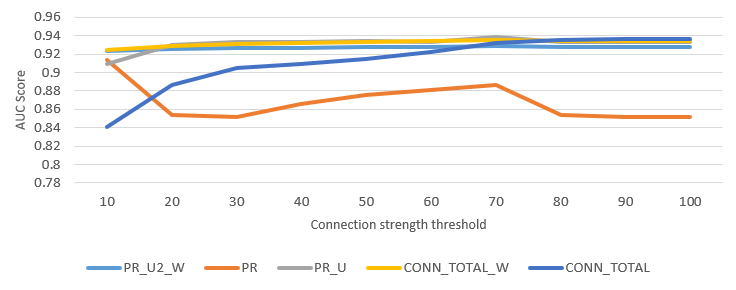
\includegraphics[width=\columnwidth]{ant_SD_LD.PNG}
\caption{Variation of AUC score when varying connection strength threshold for Ant. Results for structural and logical dependencies combined. }
\label{fig:plot_sd_ld_ant}
\centering
\end{figure}


\begin{figure}[H]
\centering
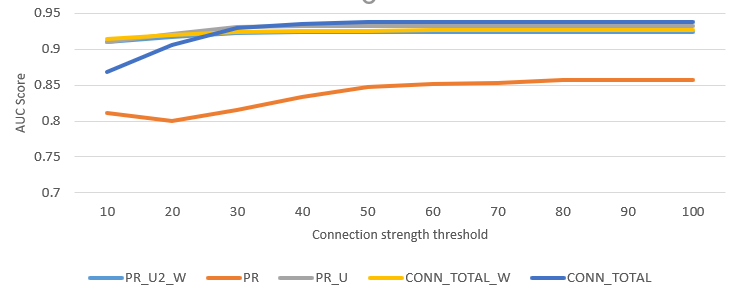
\includegraphics[width=\columnwidth]{tomcat_SD_LD.PNG}
\caption{Variation of AUC score when varying connection strength threshold for Tomcat. Results for structural and logical dependencies combined. }
\label{fig:plot_sd_ld_tomcat}
\centering
\end{figure}


\begin{figure}[H]
\centering
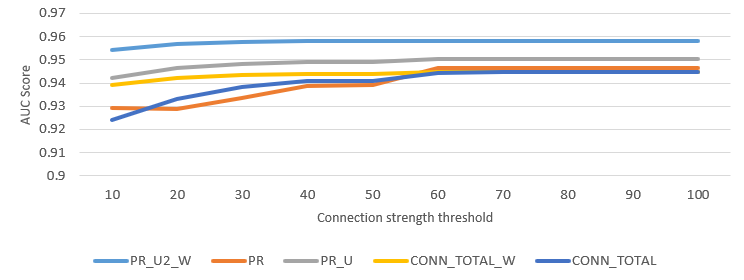
\includegraphics[width=\columnwidth]{hibernate_SD_LD.PNG}
\caption{Variation of AUC score when varying connection strength threshold for Hibernate. Results for structural and logical dependencies combined. }
\label{fig:plot_sd_ld_hibernate}
\centering
\end{figure}



\begin{figure}[H]
\centering
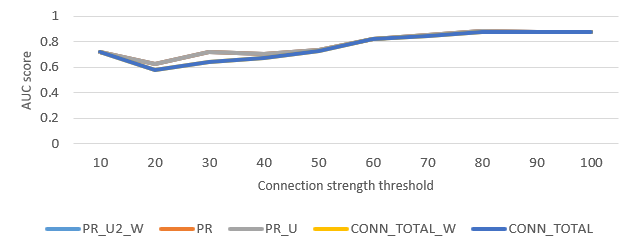
\includegraphics[width=\columnwidth]{ant_LD.PNG}
\caption{Variation of AUC score when varying connection strength threshold for Ant. Results for logical dependencies only. }
\label{fig:plot_ld_ant}
\centering
\end{figure}


\begin{figure}[H]
\centering
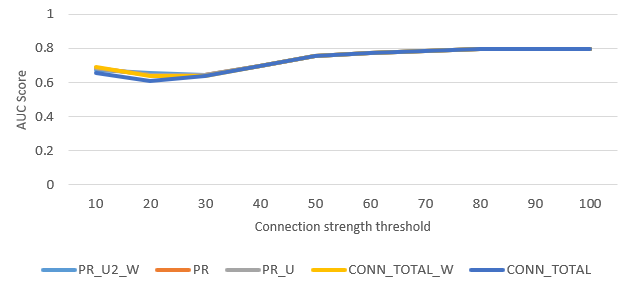
\includegraphics[width=\columnwidth]{tomcat_LD.PNG}
\caption{Variation of AUC score when varying connection strength threshold for Tomcat. Results for logical dependencies only. }
\label{fig:plot_ld_tomcat}
\centering
\end{figure}


\begin{figure}[H]
\centering
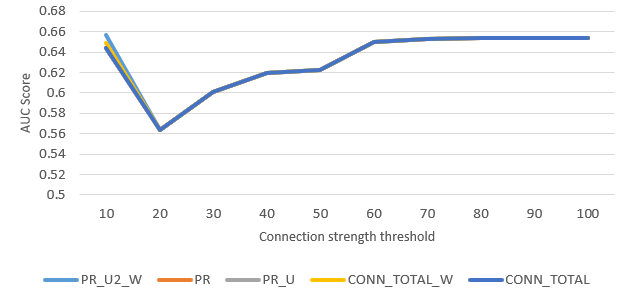
\includegraphics[width=\columnwidth]{hibernate_LD.PNG}
\caption{Variation of AUC score when varying connection strength threshold for Hibernate. Results for logical dependencies only.}
\label{fig:plot_ld_hibernate}
\centering
\end{figure}


The details of the systems are presented in two tables.  In table \ref{tab:overlap} are the overlappings between structural and logical dependencies expressed in percentages. Each column represents the percentage of logical dependencies that are also structural, for each column the logical dependencies are obtained by applying a different connection strength filter. The connection strength filter begins at 10, meaning that in at least 10 \% of the total commits involving two entities, the entities update together. We increase the connection strength filter by 10 up until we reach 100, meaning that in all the commits that involve one entity, the other entity is present also.


In table \ref{tab:ratio_sd_ld} are the ratio numbers between structural dependencies and logical dependencies. We added this table in order to highlight how different the total number of both dependencies is.


\begin{table}[!h]
\renewcommand{\arraystretch}{1}
\caption{Percentage of logical dependencies that are also structural dependencies}
\label{tab:overlap}
\centering
\scalebox{0.7}{
\begin{tabular}{|c|cccccccccc|}
\hline
System &	$\geq10\%$	&	$\geq20\%$		&	$\geq30\%$		&	$\geq40\%$		&	$\geq50\%$		&	$\geq60\%$		&	$\geq70\%$		&	$\geq80\%$		&	$\geq90\%$		&	$\geq100\%$ \\
\hline
Ant	&	25.202	&	34.419	&	36.385	&	34.656	&	33.528	&	33.333	&	28.659	&	33.333	&	35.294	&	35.294	\\
Tomcat Catalina	&	4.059	&	22.089	&	25.000	&	25.758	&	25.926	&	37.525	&	47.368	&	55.285	&	75.000	&	76.923	\\
Hibernate	&	6.546	&	26.607	&	29.565	&	32.374	&	32.543	&	45.170	&	44.980	&	42.473	&	42.473	&	42.473	\\
\hline
\end{tabular}
}
\end{table}



\begin{table}[!h]
\renewcommand{\arraystretch}{1}
\caption{Ratio between structural and logical dependencies (SD/LD)}
\label{tab:ratio_sd_ld}
\centering
\scalebox{0.7}{
\begin{tabular}{|c|cccccccccc|}
\hline
System &	$\geq10\%$	&	$\geq20\%$		&	$\geq30\%$		&	$\geq40\%$		&	$\geq50\%$		&	$\geq60\%$		&	$\geq70\%$		&	$\geq80\%$		&	$\geq90\%$		&	$\geq100\%$ \\
\hline
Ant	&	1.315	&	3.284	&	4.972	&	5.603	&	6.175	&	10.697	&	12.915	&	27.154	&	41.529	&	41.529	\\
Tomcat Catalina	&	0.120	&	0.923	&	1.313	&	1.531	&	1.619	&	3.177	&	7.092	&	13.146	&	67.375	&	124.385	\\
Hibernate	&	1.037	&	6.391	&	10.037	&	14.947	&	18.940	&	54.248	&	83.442	&	111.704	&	111.704	&	111.704	\\

\hline
\end{tabular}
}
\end{table}

In figures \ref{fig:plot_sd_ld_ant}, \ref{fig:plot_sd_ld_tomcat} and \ref{fig:plot_sd_ld_hibernate} are the measurements obtained by using structural and logical dependencies combined. 
In all three figures, the measurements at the beginning are smaller than the rest. Once with the increasing of the threshold value also the measurements begin to increase. Meaning that better results for key class detection are found. 
The best measurements are when the threshold value is between 40 and 60, after that, the measurements tend to decrease a little bit and stay at that fixed value. 

A possible explanation of the results fluctuation and then capping is that if we are looking at table \ref{tab:ratio_sd_ld} we can see that at the beginning, the total number of logical dependencies used is close to the number of existing structural dependencies. The high volume of logical dependencies introduced might cause an erroneous detection of the key classes, in consequence, smaller measurements. 
When the threshold begins to be more restrictive and the total number of logical dependencies used begins to decrease, the key classes detection starts to improve. This improvement stops after the threshold value reaches 60\%. If we look again at table \ref{tab:ratio_sd_ld} we can see that after 60\% the number of structural dependencies outnumbers the number of logical dependencies up to 124 times in some cases. In addition, if we look at table \ref{tab:overlap} we can see that the remaining logical dependencies overlap a lot with the structural dependencies, so we are not introducing too much new information.

 So, the number of logical dependencies used is so small that it doesn't influence the key class identification. Since the structural dependencies used don't change, we obtain the same results for different threshold values. 



In figures \ref{fig:plot_ld_ant}, \ref{fig:plot_ld_tomcat} and \ref{fig:plot_ld_hibernate} are the measurements obtained by using only logical dependencies.
Initially, we expected to see a Gaussian curve, but instead, we see a bell curve.  We think that in the beginning, we use a high number of logical dependencies in key class detection, among those logical dependencies is an important number of key classes and also an important number of other classes. But the number of other classes does not influence the key classes detection. When we start to increase the value of the threshold and filter more the logical dependencies, we also filter some of the initial detected key classes and remain with a significant number of other classes. In this case, the other classes that remain influence the measurements, causing the worst-performing solutions. 
Some of the key classes are strongly connected in the versioning system, and even for higher threshold values don't get filtered out. Meanwhile, the rest of the classes that are not key classes get filtered out for higher threshold values which leads to better performing measurements when the threshold value are above 60\%. 

\subsection{Comparison between strength versus confidence metric}
\label{sec:measure_metrics}


As mentioned in section \ref{strength_filter}, we did not use the confidence metric because it does not consider the big picture of the system.
A co-changing pair $A \rightarrow B$, where A updates only once in the entire history, and when it updates, it updates together with B, will have the best confidence value that we can get. This is why we introduced the strength metric, to balance the metric in the favor of those which update more frequently.
Since both metrics require the same inputs and only the calculation method is different, we computed with our tool the confidence metric and applied the same threshold to it as to the strength metric. The only difference from how other authors computed the metric is that we multiplied its value by 100. So, the confidence values can fluctuate between 0 and 100.
In the graph used by the key classes detection tool, the structural dependencies weights are supraunitary values. So, we multiplied with 100 the confidence value to scale it to the structural dependencies weights. Otherwise, if we add a subunitary value (confidence value) to a high value (the structural weight), it will not make a difference, so we will not be able to see the impact of the logical dependencies in the graph.

\begin{table}[!h]
\setlength\tabcolsep{3.5pt}
\caption{ Average results obtained with strength versus confidence metric.}
\label{tab:confidence_vs_strength}
\centering
\scalebox{0.85}{
\begin{tabular}{|c|c|c|}
\hline
Metric  &\multicolumn{2}{c|}{Using}\\
 used &Only logical dependencies 	&	Structural and logical dependencies 	 \\
\hline
\multicolumn{3}{|c|}{Average values obtained for all systems}\\
\hline
strength	&	0.791	&	0.916	\\
confidence	&	0.731	&	0.893	\\
\hline
\multicolumn{3}{|c|}{Average values obtained for Ant}\\
\hline
strength	&	0.826	&	0.903	\\
confidence	&	0.741	&	0.873	\\
\hline
\multicolumn{3}{|c|}{Average values obtained for Tomcat Catalina}\\
\hline
strength	&	0.816	&	0.910	\\
confidence	&	0.752	&	0.878	\\
\hline
\multicolumn{3}{|c|}{Average values obtained for Hibernate}\\
\hline
strength	&	0.732	&	0.935	\\
confidence	&	0.699	&	0.929	\\
\hline
\end{tabular}
}
\end{table}


The comparison between the average values obtained by using the confidence metric and the strength metric can be found in table \ref{tab:confidence_vs_strength}.

These results help us answer the third research question: \textit{RQ3: Does the connection strength filter has a favorable impact on the detection of key classes?}. As we expected in our initial hypothesis and now based on the results, we can say that the connection strength metric is more suited for logical dependencies detection. So, by considering the mean update frequency of the entire system in the filtering process, we improve the detection of logical dependencies.


\subsection{Comparison with fan-in and fan-out metric}
\label{subsec:key_metrics}

Fan-in and fan-out are coupling metrics. The fan-in of entity A is the total number of entities that call functions of A. The fan-out of A is the total number of entities called by A \cite{5507329}.


In tables \ref{tab:measurementsfan:ant}, \ref{tab:measurementsfan:catalina}, and \ref{tab:measurementsfan:hibernate} we can find the metrics detalis for each documented key class of each system.
The first column represents the name of each key class, the second column represents the fan\_in values for each key class, the third column represents the fan\_out values, the fourth column represents the number of entities that call functions of that key class plus the number of entities that are called by the key class (fan\_in and fan\_out combined), and the fifth column represents the number of logical dependencies in which an entity is involved. 

For Ant, we can see in table \ref{tab:measurementsfan:ant} that all the key classes have logical dependencies with other classes. The LD\_NUMBER means the number of logical dependencies of an entity. The key classes with the most LD number are Project and IntrospectionHelper, these two entities can be found also in table \ref{tab:measurementstop:ant} in which we did a top 10 entities that have a logical dependency with other entities. This means that some key classes are involved in software change quite often and can be observed via system history.

\begin{table}[!h]
\renewcommand{\arraystretch}{1}
\caption{Measurements for Ant key classes}
\label{tab:measurementsfan:ant}
\centering
\scalebox{0.8}{
\begin{tabular}{|c|ccccc|}
\hline
Nr.	&	Classname	&	FAN\_IN	&	FAN\_OUT	&	FAN\_TOTAL	&	LD\_NUMBER\\
\hline
1	&	Project	&	191	&	23	&	214	&	157	\\
2	&	Target	&	28	&	6	&	34	&	78	\\
3	&	UnknownElement	&	17	&	13	&	30	&	90	\\
4	&	RuntimeConfigurable	&	17	&	13	&	30	&	118	\\
5	&	IntrospectionHelper	&	18	&	24	&	42	&	143	\\
6	&	Main	&	1	&	13	&	14	&	82	\\
7	&	TaskContainer	&	11	&	1	&	12	&	21	\\
8	&	ProjectHelper2\$ElementHandler	&	1	&	12	&	13	&	30	\\
9	&	Task	&	110	&	7	&	117	&	88	\\
10	&	ProjectHelper	&	16	&	8	&	24	&	101	\\
\hline
\end{tabular}
}
\end{table}


For Tomcat Catalina, same as for Ant, we can see in table \ref{tab:measurementsfan:catalina} that all the key classes have logical dependencies.  The key classes with the most LD number are StandardContext and Request, these two entities can also be found in table \ref{tab:measurementstop:catalina} in which we did a top 10 entities that have the most logical dependencies with other entities for Tomcat Catalina.

For Hibernate things are a little bit different, as we can see in table \ref{tab:measurementsfan:hibernate},  key classes like Criterion, Projection, or Transaction have 0 logical dependencies, meaning that those key classes are not involved in any software change. One possible explanation for this is that for Hibernate the architecture is designed in such way that the core is not often touched by change. 


\begin{table}[!h]
\renewcommand{\arraystretch}{1}
\caption{Measurements for Tomcat Catalina key classes.}
\label{tab:measurementsfan:catalina}
\centering
\scalebox{0.8}{
\begin{tabular}{|c|ccccc|}
\hline
Nr.	&	Classname	&	FAN\_IN	&	FAN\_OUT	&	FAN\_TOTAL	&	LD\_NUMBER \\
\hline
1	&	Context	&	74	&	8	&	82	&	126	\\
2	&	Request	&	48	&	28	&	76	&	215	\\
3	&	Container	&	51	&	8	&	59	&	64	\\
4	&	Response	&	38	&	12	&	50	&	90	\\
5	&	StandardContext	&	11	&	38	&	49	&	216	\\
6	&	FANector	&	23	&	9	&	32	&	89	\\
7	&	Session	&	29	&	2	&	31	&	28	\\
8	&	Valve	&	29	&	2	&	31	&	19	\\
9	&	Wrapper	&	29	&	1	&	30	&	36	\\
10	&	Manager	&	25	&	3	&	28	&	31	\\
11	&	Host	&	26	&	1	&	27	&	44	\\
12	&	Service	&	20	&	6	&	26	&	51	\\
13	&	Engine	&	23	&	2	&	25	&	1	\\
14	&	Realm	&	18	&	6	&	24	&	21	\\
15	&	CoyoteAdapter	&	1	&	22	&	23	&	140	\\
16	&	StandardHost	&	8	&	15	&	23	&	88	\\
17	&	LifecycleListener	&	21	&	1	&	22	&	3	\\
18	&    StandardEngine	&	2	&	19	&	21	&	57	\\
19	&	Pipeline	&	19	&	2	&	21	&	20	\\
20	&	Server	&	16	&	4	&	20	&	49	\\
21	&	HostConfig	&	3	&	15	&	18	&	79	\\
22	&	StandardWrapper	&	5	&	13	&	18	&	92	\\
23	&	StandardService	&	3	&	12	&	15	&	81	\\
24	&	Catalina	&	2	&	13	&	15	&	94	\\
25	&	Loader	&	14	&	1	&	15	&	18	\\
26	&	StandardServer	&	2	&	12	&	14	&	94	\\
27	&	StandardPipeline	&	1	&	10	&	11	&	62	\\
28	&	Bootstrap	&	3	&	3	&	6	&	41	\\	
\hline
\end{tabular}
}
\end{table}

\begin{table}[!h]
\renewcommand{\arraystretch}{1}
\caption{Measurements for Hibernate key classes.}
\label{tab:measurementsfan:hibernate}
\centering
\scalebox{0.8}{
\begin{tabular}{|c|ccccc|}
\hline
Nr.	&	Classname	&	FAN\_IN	&	FAN\_OUT	&	FAN\_TOTAL	&	LD\_NUMBER \\
\hline
1	&	SessionFactoryImplementor	&	438	&	43	&	481	&	51	\\
2	&	Type	&	444	&	5	&	449	&	0	\\
3	&	Table	&	89	&	29	&	118	&	82	\\
4	&	SessionImplementor	&	52	&	12	&	64	&	14	\\
5	&	Criteria	&	45	&	12	&	57	&	15	\\
6	&	Column	&	46	&	10	&	56	&	20	\\
7	&	Session	&	31	&	21	&	52	&	52	\\
8	&	Query	&	12	&	28	&	40	&	0	\\
9	&	Configuration	&	1	&	38	&	39	&	115	\\
10	&	SessionFactory	&	24	&	12	&	36	&	33	\\
11	&	Criterion	&	30	&	3	&	33	&	0	\\
12	&	Projection	&	11	&	3	&	14	&	0	\\
13	&	FANectionProvider	&	12	&	2	&	14	&	0	\\
14	&	Transaction	&	11	&	1	&	12	&	0	\\
				
\hline
\end{tabular}
}
\end{table}


%%%%%%%%%%%%%%%%%%%%%%%%%%%%%%%%%%%%%%%%%%%%%%%%%%%%%%%%%%%%%%%%%%%%%%%%%%%%%

In tables \ref{tab:measurementstop:ant}, \ref{tab:measurementstop:catalina}, and \ref{tab:measurementstop:hibernate} we can find the top 10 entities with logical dependencies. The first column represents the name of each top 10 entity, the second column represents the fan\_in values, the third column represents the fan\_out values, the fourth column represents the fan\_in and fan\_out combined, and the fifth column represents the number of logical dependencies in which the entity is involved.


We did these top 10 tables to offer an overview of the highest registered numbers for LD for each system. As we mentioned before, some of the key classes are also present in these tables, but not all of them.

In table \ref{tab:measurementstop:hibernate} we can find the top 10 measurements for Hibernate, most of the table is occupied by inner classes of AbstractEntityPersister. This is expected behavior since class AbstractEntityPersister is also present. This behavior is caused by the impossibility to separate the updates done for a class from its inner classes in the versioning system. So, each time AbstractEntityPersister records a change, also the inner classes are considered to have changed.
\begin{table}[!h]
\renewcommand{\arraystretch}{1}
\caption{Top 10 measurements for Ant. }
\label{tab:measurementstop:ant}
\centering
\scalebox{0.8}{
\begin{tabular}{|c|ccccc|}
\hline
Nr.	&	Classname	&	FAN\_IN	&	FAN\_OUT	&	FAN\_TOTAL	&	LD\_NUMBER \\
\hline
1	&	\cellcolor{lightorange}Project	&	191	&	23	&	214	&	157	\\
2	&	Project\$AntRefTable	&	1	&	2	&	3	&	157	\\
3	&	Path	&	39	&	13	&	52	&	147	\\
4	&	Path\$PathElement	&	3	&	2	&	5	&	147	\\
5	&	\cellcolor{lightorange}IntrospectionHelper	&	18	&	24	&	42	&	143	\\
6	&	IntrospectionHelper\$AttributeSetter	&	8	&	1	&	9	&	143	\\
7	&	IntrospectionHelper\$Creator	&	3	&	5	&	8	&	143	\\
8	&	IntrospectionHelper\$NestedCreator	&	7	&	1	&	8	&	143	\\
9	&	Ant	&	2	&	15	&	17	&	136	\\
10	&	Ant\$Reference	&	3	&	1	&	4	&	136	\\
\hline
\end{tabular}
}
\end{table}

\begin{table}[!h]
\renewcommand{\arraystretch}{1}
\caption{Top 10 measurements for Tomcat Catalina. }
\label{tab:measurementstop:catalina}
\centering
\scalebox{0.8}{
\begin{tabular}{|c|ccccc|}
\hline
Nr.	&	Classname	&	FAN\_IN	&	FAN\_OUT	&	FAN\_TOTAL	&	LD\_NUMBER \\
\hline
1	&	\cellcolor{lightorange}StandardContext	&	11	&	38	&	49	&	216	\\
2	&	StandardContext\$ContextFilterMaps	&	0	&	0	&	0	&	216	\\
3	&	StandardContext\$NoPluggabilityServletContext	&	0	&	0	&	0	&	216	\\
4	&	\cellcolor{lightorange}Request	&	48	&	28	&	76	&	215	\\
5	&	Request\$SpecialAttributeAdapter	&	0	&	0	&	0	&	215	\\
6	&	ApplicationContext	&	3	&	22	&	25	&	158	\\
7	&	ApplicationContext\$DispatchData	&	0	&	0	&	0	&	158	\\
8	&	ContextConfig	&	3	&	26	&	29	&	143	\\
9	&	ContextConfig\$DefaultWebXmlCacheEntry	&	0	&	0	&	0	&	143	\\
10	&	ContextConfig\$JavaClassCacheEntry	&	0	&	0	&	0	&	143	\\
\hline
\end{tabular}
}
\end{table}


\begin{table}[!h]
\renewcommand{\arraystretch}{1}
\caption{Top 10 measurements for Hibernate. }
\label{tab:measurementstop:hibernate}
\centering
\scalebox{0.8}{
\begin{tabular}{|c|ccccc|}
\hline
Nr.	&	Classname	&	FAN\_IN	&	FAN\_OUT	&	FAN\_TOTAL	&	LD\_NR \\
\hline
1	&	AvailableSettings	&	1	&	0	&	1	&	205	\\
2	&	AbstractEntityPersister	&	9	&	143	&	152	&	190	\\
3	&	AbstractEntityPersister\$CacheEntryHelper	&	0	&	0	&	0	&	190	\\
4	&	AbstractEntityPersister\$InclusionChecker	&	0	&	0	&	0	&	190	\\
5	&	AbstractEntityPersister\$NoopCacheEntryHelper	&	0	&	0	&	0	&	190	\\
6	&	AbstractEntityPersister\$ReferenceCacheEntryHelper	&	0	&	0	&	0	&	190	\\
7	&	AbstractEntityPersister\$StandardCacheEntryHelper	&	0	&	0	&	0	&	190	\\
8	&	AbstractEntityPersister\$StructuredCacheEntryHelper	&	0	&	0	&	0	&	190	\\
9	&	Dialect	&	265	&	104	&	369	&	176	\\
10	&	SessionFactoryImpl\$SessionBuilderImpl	&	1	&	25	&	26	&	167	\\
\hline
\end{tabular}
}
\end{table}

Overall, by looking at the comparisons between FAN\_IN, FAN\_OUT, FAN\_TOTAL, and the logical dependencies in which a class is involved we could not determine a direct connection between them. Nither we can say that one influences the other.  We consider that even though the metrics are not related directly, they could be all used together to get a better view of the system connections.



\section{Chapter conclusions}
\label{sec:key_class_conclusions}

In this paper, we studied the filtering and the usage of co-changes extracted from the versioning system. In the first part of the paper, we focused on the co-changes filtering, and in the second part, we used the filtered co-changes (logical dependencies) to detect key classes.
For co-changes filtering, we applied the commit size filter and the filter based on connection strength. The co-changes that remained after filtering, called logical dependencies, were provided as input for a tool that detects key classes. 

We approached two scenarios to detect key classes by using logical dependencies. In the 1$^{st}$ scenario, we used logical dependencies together with structural dependencies, and in the 2$^{nd}$, we used only logical dependencies to detect the key classes. We modified the tool used in the baseline approach for detecting key classes from structural dependencies \cite{Finding-key-classes}, to use also logical dependencies.

Based on the results obtained, compared with the baseline results, we saw a slight improvement in key class detection when both logical and structural dependencies were used together. The best results were obtained with a connection strength threshold of 40-70. Also, our connection strength metric performs better than the confidence metric used in related works.

When we used only logical dependencies to detect key classes, the results were less performing than our results when using only structural or structural and
logical dependencies combined, but they were comparable with results of related work using structural dependencies. We consider this a very
positive result because this research uses a different type of input than the previous ones, the logical dependencies.
It is also an open door for new research in multiple fields that use structural dependencies to gain knowledge about software systems. And since logical dependencies are easy and fast to extract from the versioning system and do not depend on the language of the software system, the cost of integrating them is small. 

To sum up the findings of this paper, logical dependencies can be used to gain knowledge about software systems. We consider that the advantage of using only logical dependencies is that it only uses data extracted from the versioning system and can be generalized to various programming languages.

In the future, we want to check if other areas can be improved by using logical dependencies, like software clustering \cite{SoraConti}, \cite{Shtern:2012:CMS:2332427.2332428}, \cite{SoraSem13}.